\documentclass{article}
\usepackage[paperwidth=4.2in,paperheight=4.2in,margin=0.1in]{geometry}
\usepackage{tikz}
\usetikzlibrary{shapes,arrows.meta,decorations.pathmorphing}
\definecolor{boxblue}{RGB}{45,90,150}
\definecolor{boxteal}{RGB}{30,120,120}
\definecolor{boxorange}{RGB}{210,110,30}
\definecolor{warnred}{RGB}{220,60,60}
\pagestyle{empty}
\begin{document}
\begin{center}
\vspace*{\fill}
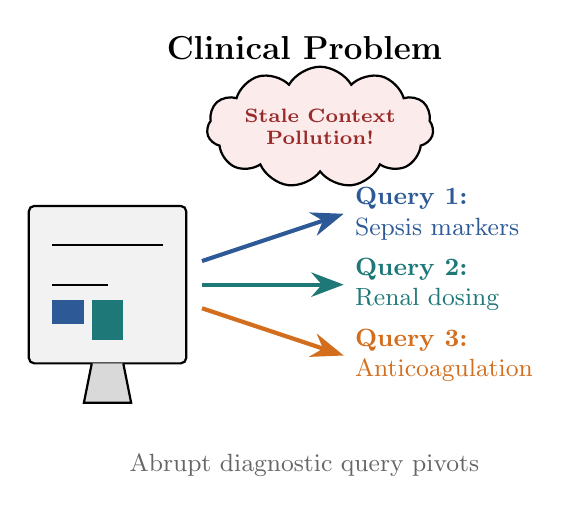
\begin{tikzpicture}[font=\sffamily]
% Title
\node[font=\large\bfseries] at (1.0, 3.5) {Clinical Problem};

% Cloud (Now safely at the top)
\node[cloud, cloud puffs=11, cloud puff arc=120, aspect=2.5, draw, thick, fill=warnred!10, text=warnred!70!black, font=\scriptsize\bfseries, align=center, inner sep=1pt] at (1.2, 2.5) {Stale Context\\Pollution!};

% EHR Monitor
\draw[thick, fill=gray!10, rounded corners=2pt] (-2.5, -0.5) rectangle (-0.5, 1.5);
\draw[thick, fill=gray!30] (-1.7, -0.5) -- (-1.8, -1) -- (-1.2, -1) -- (-1.3, -0.5);
\draw[thick] (-2.2, 1.0) -- (-0.8, 1.0);
\draw[thick] (-2.2, 0.5) -- (-1.5, 0.5);
\fill[boxblue] (-2.2, 0) rectangle (-1.8, 0.3);
\fill[boxteal] (-1.7, -0.2) rectangle (-1.3, 0.3);

% Queries
\draw[-{Stealth[scale=1.2]}, line width=1.5pt, boxblue] (-0.3, 0.8) -- (1.5, 1.4) node[right, align=left, font=\small] {\textbf{Query 1:}\\Sepsis markers};
\draw[-{Stealth[scale=1.2]}, line width=1.5pt, boxteal] (-0.3, 0.5) -- (1.5, 0.5) node[right, align=left, font=\small] {\textbf{Query 2:}\\Renal dosing};
\draw[-{Stealth[scale=1.2]}, line width=1.5pt, boxorange] (-0.3, 0.2) -- (1.5, -0.4) node[right, align=left, font=\small] {\textbf{Query 3:}\\Anticoagulation};

% Bottom Text
\node[align=center, font=\small, text=gray!80!black] at (1.0, -1.8) {Abrupt diagnostic query pivots};
\end{tikzpicture}
\vspace*{\fill}
\end{center}
\end{document}
